\documentclass{article}

% Package `amsthm` and `thmtools` must come before package `hyperref`.
\usepackage{amsthm}
\usepackage{thmtools}
% Package `hyperref` must come before package `complexity`.
\usepackage[pdftitle={Complexity of computing the size of the minimum generating set of a group}, pdfauthor={Jeffrey Finkelstein}]{hyperref}
\usepackage{complexity}
\usepackage{amsmath}
\usepackage{amssymb}
\usepackage{tikz}

\newcommand{\gen}[1]{{\langle #1 \rangle}}
\newcommand{\email}[1]{\href{mailto:#1}{\nolinkurl{#1}}}

\declaretheorem[numberwithin=section]{theorem}
\declaretheorem[numberlike=theorem]{conjecture}
\declaretheorem[numberlike=theorem]{lemma}
\declaretheorem[numberlike=theorem]{proposition}
\declaretheorem[numberlike=theorem, style=definition]{definition}
\declaretheorem[numberlike=theorem, style=definition]{todo}

\title{Complexity of computing the size of the minimum generating set of a group}
\author{Jef{}frey~Finkelstein}
\date{\today}

\begin{document}
\maketitle

\section{Introduction}

In this work we study the problem of computing the size of the minimum generating set of a group when given as a Cayley table, as well as the restriction of this problem to restricted classes of groups.
Previously, the best upper bound for this problem was $\L^2$ (also known as $\DSPACE(\log^2 n)$), due to \cite{lsz77} (also described in \cite[Proposition~3]{at06}).
The more recent work by many authors on ``bounded nondeterminism'' (in which an algorithm is allowed to nondeterministically guess a limited amount of bits and then verify the guess deterministically) as well as improved algorithms for deciding group membership due to \cite{bm89} and \cite{bklm01} allow us to improve this upper bound to $\GC(\log^2 n, \L)$ (defined in \autoref{sec:prelim}) using a more careful analysis of the original $\L^2$ algorithm.

The related problem of deciding group membership was placed in $\L^2$ by \cite{lsz77}, and later improved to \SL{} by \cite{bm89}.
In \cite{bklm01}, the group membership problem for several restricted classes of groups was placed in \FOLL, a class similar to $\AC^0$ but with $O(\log \log n)$ depth.
The more recent proof that $\SL = \L$ \cite{reingold08} places the membership problem for general groups (and thus for restricted classes of groups) squarely in \L.

Also related is the problem of deciding whether two given groups are isomorphic.
A series of works improved the upper bound for the \emph{quasi}group isomorphism problem (and hence the group isomorphism problem) from $\GC(\log^2 n, \P)$ \cite{py96} to $\GC(\log^2 n, \NC^2)$ \cite{wolf94} to $\GC(\log^2 n, \SAC^1)$ \cite{wagner10} to $\GC(\log^2 n, \FOLL)$ \cite{ctw10}.

\section{Preliminaries}\label{sec:prelim}

Throughout this work, $\log n$ denotes the base 2 logarithm of $n$.

\P{} is the class of decision problems decidable by a deterministic Turing machine halting in polynomial time.
$\L^2$ is the class of decision problems decidable by a deterministic Turing machine using at most $O(\log^2 n)$ space.
The (inclusion) relationship between \P{} and $\L^2$ is unknown.
\FOLL{} is the class of decision problems decidable by a $\DTIME(\log n)$-uniform family of circuits with polynomial size, unbounded fan-in, and $O(\log \log n)$ depth.
$\FOLL^2$ is the same, but with $O(\log^2 \log n)$.
Following the notation of Cai and Chen \cite{cc97}, $\GC(f(n), \mathcal{C})$ is the class of decision problems decidable by a $\mathcal{C}$ machine augmented with $O(f(n))$ nondeterministic bits.
We will consider specifically the complexity classes $\GC(\log^2 n, \L)$ and $\GC(\log^2 n, \FOLL)$.

Let $P$ and $Q$ be decision problems.
We say \emph{$P$ is many-one reducible to $Q$} if there exists a function $f$ such that for all strings $x$, we have $x \in P$ if and only if $f(x) \in Q$.

If $(G, \cdot)$ is a finite group of order $n$, we identify the elements of the group with the indices 1, 2, \ldots, n, where 1 is the identity of the group.
We sometimes refer to the group as $(G, \cdot)$, but will also sometimes omit the group product and just write $G$.
The \emph{Cayley table} of this group is the $n \times n$ matrix with entries from $G$ in which entry $(u, v)$ has value $g$ if $u \cdot g = v$.
We will consider all elements of $G$ to be expressed in binary, so the size of each element of $G$ is $\log n$ and the size of the Cayley table is $n^2 \log n$.
If $T \subseteq G$, the set \emph{generated} by $T$, denoted $\gen{T}$, is the transitive closure of $\cdot$ on $T$.
A \emph{generating set} for $(G, \cdot)$ is a set $T \subseteq G$ such that $\gen{T} = G$.

We will also consider subclasses of the class of all \emph{finite} groups: \textsc{Group}, \textsc{Constant Solvability Class}, \textsc{Nilpotent}, \textsc{Abelian}, \textsc{p-Group}, \textsc{Elementary Abelian}, and \textsc{Cyclic}, where \textsc{Group} is the class of all finite groups, \textsc{Constant Solvability Class} is the class of all finite groups of solvability class $O(1)$, etc.
Inclusions among these classes are given in \autoref{fig:inclusions}.
\begin{figure}
  \caption{Inclusions among classes of finite groups.\label{fig:inclusions}}
  \begin{center}
    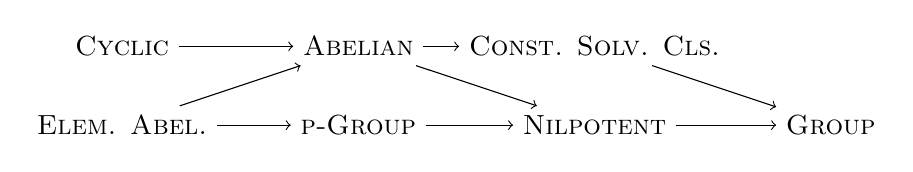
\begin{tikzpicture}[xscale=3]

      \node (e) at (0, 0) {\textsc{Elem. Abel.}};
      \node (c) at (0, 1) {\textsc{Cyclic}};
      \node (p) at (1, 0) {\textsc{p-Group}};
      \node (a) at (1, 1) {\textsc{Abelian}};
      \node (n) at (2, 0) {\textsc{Nilpotent}};
      \node (s) at (2, 1) {\textsc{Const. Solv. Cls.}};
      \node (g) at (3, 0) {\textsc{Group}};

      \path[->]
      (c) edge (a)
      (e) edge (a)
      (e) edge (p)

      (a) edge (s)
      (a) edge (n)
      (p) edge (n)

      (s) edge (g)
      (n) edge (g);
    \end{tikzpicture}
  \end{center}
\end{figure}

\section{Decision problem for computing the size of the minimum generating set}

In order to study the complexity of computing the size of the minimum generating set, we define a decision problem corresponding to this optimization problem.

\begin{definition}[\textsc{Min Gen Size($\mathcal{G}$)}]
  \mbox{}

  \textbf{Instance:} finite group $(G, \cdot)$ (given as a Cayley table) in the class $\mathcal{G}$, natural number $k$ (given in binary).

  \textbf{Question:} Does there exist a $T \subseteq G$ such that $\gen{T} = G$ and $|T| \leq k$?
\end{definition}

Since each of the other classes of groups is a subclass of \textsc{Group}, an upper bound on the complexity of \textsc{Min Gen Size(Group)} is also an upper bound on the complexity of \textsc{Min Gen Size} for all the other subclasses.

Previously, the \textsc{Min Gen Size(Group)} problem was known to be in $\L^2$, the class of problems decidable by a deterministic Turing machine using at most $O(\log^2 n)$ space \cite{lsz77} (see \cite[Proposition~3]{at06} for a brief description of the algorithm; I can't find a copy of \cite{lsz77} online).
We can improve this upper bound by a more careful analysis of the $\L^2$ algorithm using the following auxiliary decision problem.

\begin{definition}[\textsc{Membership($\mathcal{G}$)}]
  \mbox{}

  \textbf{Instance:} finite group $(G, \cdot)$ (given as a Cayley table) in the class $\mathcal{G}$, finite set $S \subset G$, group element $v \in G$.

  \textbf{Question:} Is $v \in \gen{S}$?
\end{definition}

\begin{lemma}\label{lem:membershipinl}
  $\textsc{Membership(Group)} \in \L$.
\end{lemma}
\begin{proof}
  Since $\textsc{Membership(Group)} \in \SL$ \cite[Section~3]{bm89}, and $\SL = \L$ \cite{reingold08}, the lemma follows.
\end{proof}

Upper bounds on the complexity of \textsc{Membership($\mathcal{G}$)} for several subclasses of \textsc{Group} are explored in \cite{bklm01}.
%We use the logarithmic space algorithm for this problem to give a simple $\GC(\log^2 n, \L)$ algorithm for \textsc{Min Group Gen}.

Before providing the general algorithms for computing the size of the minimum generating set for classes of groups, we require one algebraic lemma which bounds the size of the minimum generating set of any finite group.

\begin{lemma}\label{lem:log}
  If $(G, \cdot)$ is a finite group then the size of the minimum generating set is at most $\log n$.
\end{lemma}
\begin{proof}
  Proof can be found at \url{http://math.stackexchange.com/a/226938/29369}, add it here.
\end{proof}

This lemma allows us to consider, without loss of generality, only inputs $\langle (G, \cdot), k \rangle$ such that $k \leq \log n$.

\subsection{In logarithmic space with bounded nondeterminism}

\begin{theorem}\label{thm:mingengc}
  $\textsc{Min Gen Size(Group)} \in \GC(\log^2 n, \L)$.
\end{theorem}
\begin{proof}
  The algorithm proceeds as follows on input $\langle (G, \cdot), k \rangle$, where $G$ is a group of order $n$:
  \begin{itemize}
  \item Nondeterministically guess a subset $S \subseteq G$ of cardinality at most $k$.
  \item Accept if and only if for all $v \in G$, $\langle G, S, v \rangle \in \textsc{Membership(Group)}$.
  \end{itemize}

  First we prove that this algorithm uses $O(\log^2 n)$ nondeterministic bits and $O(\log n)$ space.
  The size of each group element, represented as number in binary, is $\log n$.
  By \autoref{lem:log}, we assume without loss of generality that the size of the minimum generating set for a group of order $n$ is at most $\log n$, so $k$ must be at most $\log n$.
  Therefore the total number of nondeterministic bits required to guess $S$ is $O(\log^2 n)$.
  Iterating over all elements of $G$ requires $O(\log n)$ space to keep track of the current element in the iteration.
  Since $\textsc{Membership(Group)} \in \L$ by \autoref{lem:membershipinl}, deciding whether $\langle G, S, v \rangle \in \textsc{Membership(Group)}$ uses at most $O(\log n)$ space.
  Therefore the total space required for this algorithm (other than the read-only input and read-only nondeterministic bits) is $O(\log n)$.

  Next we show that the algorithm correctly decides the problem.
  Suppose $\langle (G, \cdot), k) \rangle \in \textsc{Min Gen Size(Group)}$, so there exists a $T \subseteq G$ such that $|T| \leq k$ and $\gen{T} = G$.
  One of the sets $S$ of cardinality at most $k$ that the algorithm guesses will equal $T$, since $|T| \leq k$.
  For all elements $v \in G$, we have $v \in \gen{T}$ since $\gen{T} = G$.
  Hence the (correct) algorithm for \textsc{Membership(Group)} will accept for all $v \in G$, and the overall algorithm will accept.
  For the converse, suppose the algorithm accepts the input $\langle (G, \cdot), k \rangle$.
  This occurs exactly when it has guessed a set $S$ of cardinality at most $k$ such that all elements $v$ in $G$ are members of the subgroup generated by $S$.
  Thus $S$ is a generating set for $G$ of cardinality at most $k$, so $\langle (G, \cdot), k \in \textsc{Min Gen Size(Group)}$.
\end{proof}

This improves the previous upper bound, $\L^2$, because
\begin{equation*}
  \GC(\log^2 n, \L) \subseteq \GC(\log^2 n, \NC^2) \subseteq \L^2,
\end{equation*}
where the first inclusion follows from the fact that $\L \subseteq \NL \subseteq \NC^2$, and the second is proven in \cite[Lemma~3.2.8]{wolf90}.

\subsection{In \texorpdfstring{\FOLL}{FOLL} with bounded nondeterminism}

\begin{theorem}
  \mbox{}
  \begin{enumerate}
  \item Each of the problems
    \begin{itemize}
    \item \textsc{Min Gen Size(Constant Solvability Class)},
    \item \textsc{Min Gen Size(Abelian)},
    \item \textsc{Min Gen Size(Elementary Abelian)}, and
    \item \textsc{Min Gen Size(Cyclic)}
    \end{itemize}
    is in $\GC(\log^2 n, \FOLL)$.
  \item $\textsc{Min Gen Size(Nilpotent)} \in \GC(\log^2 n, \FOLL^2)$.
  \end{enumerate}
\end{theorem}
\begin{proof}
  \mbox{}
  \begin{enumerate}
  \item
    We know that the membership problem for each of these classes of groups is in \FOLL{} by \cite[Section~3]{bklm01}.
    A slight modification of the algorithm from \autoref{thm:mingengc} can be used to show that each of these problems is in $\GC(\log^2 n, \FOLL)$.
    After nondeterministically guessing a set $S$, instead of iterating over each element of the group in logarithmic space, we use $n$ instances of the \FOLL{} circuit which decides the membership problem and compute the conjunction of the output of each of the instances for one additional layer of depth and a $O(n)$ increase in the size of the circuit.
    Since the size of the circuit remains polynomial in $n$ and the depth remains $O(\log \log n)$, we have shown $\textsc{Min Gen Size(Cyclic)} \in \GC(\log^2 n, \FOLL)$.
  \item The same argument applies, except using the fact that the membership problem for nilpotent groups is in $\FOLL^2$ \cite[Corollary~3.12]{bklm01}. \qedhere
  \end{enumerate}
\end{proof}
%% Observe that even though, for example, $\textsc{Membership(Cyclic)} \in \L \cap \FOLL$, we show that \textsc{Min Gen Size(Cyclic)} is in
%% \begin{equation*}
%%   \GC(\log^2 n, \L) \cap \GC(\log^2 n, \FOLL)
%% \end{equation*}
%% instead of
%% \begin{equation*}
%%   \GC(\log^2 n, \L \cap \FOLL),
%% \end{equation*}
%% for syntactic reasons (the second step in the algorithm from \autoref{thm:mingengc} is either a logarithmic space Turing machine procedure or a $\FO(\log \log n)$ procedure, but not both simultaneously).

\subsection{In polynomial time}

In \cite{at06}, the authors provide a polynomial time conjunctive truth-table reduction from \textsc{Min Gen Size(Nilpotent)} to \textsc{Min Gen Size(Elementary Abelian)} via \textsc{Min Gen Size(p-Group)}.
They note that since there is a deterministic polynomial time algorithm for \textsc{Min Gen Size(Elementary Abelian)}, there is one for each of the others as well.
This result also implies a polynomial time algorithm for all subclasses of the the class of finite nilpotent groups.

\begin{theorem}[{\cite[Theorem~7]{at06}}]
  Each of the problems
  \begin{itemize}
  \item \textsc{Min Gen Size(Nilpotent)},
  \item \textsc{Min Gen Size(p-Group)},
  \item \textsc{Min Gen Size(Abelian)},
  \item \textsc{Min Gen Size(Elementary Abelian)}, and
  \item \textsc{Min Gen Size(Cyclic)}
  \end{itemize}
  is in \P.
\end{theorem}

A clearer presentation of the complete proof is given in \autoref{app:p}.

\subsection{In constant depth circuits}

For cyclic groups, the size of the minimum generating set is always 1, so the problem is uninteresting.

\begin{theorem}
  $\textsc{Min Gen Size(Cyclic)} \in \NC^0$.
\end{theorem}

\section{Searching for the exact size of the minimum generating set}

Now that we know the complexity for the decision problem form of \textsc{Min Gen Size(Group)}, we wish to implement a function which computes the exact size of the minimum generating set of a group.
For decision problems in polynomial time, the well-known binary search on $k$ between 1 and $n$, where $n$ is the order of the group, places the search problem in polynomial time as well.
For decision problems in $\GC(\log^2 n, \L)$, however, each level of the binary search recursion tree requires an additional $O(\log^2 n)$ bits of nondeterminism.
(The $O(\log n)$ space can still be reused at each level.)
For this reason, the search problem corresponding to \textsc{Min Gen Size(Group)} is computable in $\GC(\log^3 n, \L)$.

\begin{todo}
  How can we perform binary search in $\GC(\log^2 n, \FOLL)$?
\end{todo}

\section{Completeness}

Any decision problem in \FOLL{} (or $\FOLL^2$) cannot be hard under $\AC^0$ many-one reductions for any complexity class which contains $\textsc{Parity}$ \cite[Section~2.2]{bklm01}.
This is true even when the circuit is augmented with a polylogarithmic number of nondeterministic gates \cite[Section~4]{ctw10}.
This gives an immediate improvement to the upper bound of all the problems shown in the previous section to be in $\GC(\log^2 n, \FOLL)$ (or $\GC(\log^2 n, \FOLL^2)$).

\begin{theorem}
  None of the decision problems
  \begin{itemize}
  \item \textsc{Min Gen Size(Nilpotent)},
  \item \textsc{Min Gen Size(p-Group)},
  \item \textsc{Min Gen Size(Constant Solvability Class)},
  \item \textsc{Min Gen Size(Abelian)},
  \item \textsc{Min Gen Size(Elementary Abelian)}, or
  \item \textsc{Min Gen Size(Cyclic)}
  \end{itemize}
  are hard under $\AC^0$ many-one reductions for any complexity class containing \textsc{Parity}, specifically those in the inclusion chain
  \begin{equation*}
    \ACC^0 \subseteq \TC^0 \subseteq \NC^1 \subseteq \L \subseteq \NL \subseteq (\LOGCFL \cup \DET).
  \end{equation*}
\end{theorem}

\section{Future work}

\autoref{fig:results} contains a summary of the results found in this work.

\begin{figure}
\caption{A summary of the upper bounds due to this work for the problem of computing the size of the minimum generating set of a class of groups.\label{fig:results}}
  \begin{center}
    \begin{tabular}{l | l}
      \multicolumn{1}{c |}{Subclass $\mathcal{G}$ of \textsc{Group}}
      &
      \multicolumn{1}{| c}{\textsc{Min Gen Size($\mathcal{G}$)} decision problem} \\
      \hline
      \hline
      \textsc{Group} & $\GC(\log^2 n, \L)$ \\
      \textsc{Solvable} & $\GC(\log^2 n, \L)$ \\
      \textsc{Nilpotent} & $\GC(\log^2 n, \L) \cap \GC(\log^2 n, \FOLL^2) \cap \P$ \\
      \textsc{p-Group} & $\GC(\log^2 n, \L) \cap \GC(\log^2 n, \FOLL^2) \cap \P$ \\
      \textsc{Constant Solvability Class} & $\GC(\log^2 n, \L) \cap \GC(\log^2 n, \FOLL)$ \\
      \textsc{Abelian} & $\GC(\log^2 n, \L) \cap \GC(\log^2 n, \FOLL) \cap \P$ \\
      \textsc{Elementary Abelian} & $\GC(\log^2 n, \L) \cap \GC(\log^2 n, \FOLL) \cap \P$ \\
      \textsc{Cyclic} & $\NC^0$ \\
      \multicolumn{2}{c}{} \\[10pt]
      \multicolumn{1}{c |}{Subclass $\mathcal{G}$ of \textsc{Group}}
      &
      \multicolumn{1}{| c}{\textsc{Min Gen Size($\mathcal{G}$)} search problem} \\
      \hline
      \hline
      \textsc{Group} & $\GC(\log^3 n, \L)$ \\
      \textsc{Solvable} & $\GC(\log^3 n, \L)$ \\
      \textsc{Nilpotent} & $\GC(\log^3 n, \L) \cap \P$ \\
      \textsc{p-Group} & $\GC(\log^3 n, \L) \cap \P$ \\
      \textsc{Constant Solvability Class} & $\GC(\log^3 n, \L)$ \\
      \textsc{Abelian} & $\GC(\log^3 n, \L) \cap \P$ \\
      \textsc{Elementary Abelian} & $\GC(\log^3 n, \L) \cap \P$ \\
      \textsc{Cyclic} & $\NC^0$
    \end{tabular}
  \end{center}
\end{figure}

As noted in the introduction, the (quasi)group isomorphism problem is known to be in $\GC(\log^2 n, \FOLL)$.
What is the relationship between this problem and the minimum generating set size problem for groups?

What is the relationship between computing the size of the minimum generating set and computing the minimum generating set itself?

\section{About this work}

Copyright 2012 Jef{}frey Finkelstein.

This work is licensed under the Creative Commons Attribution-ShareAlike License 3.0.
Visit \mbox{\url{https://creativecommons.org/licenses/by-sa/3.0/}} to view a copy of this license.

The \LaTeX{} markup which generated this document is available on the World Wide Web at \mbox{\url{https://github.com/jfinkels/ncapproximation}}.
It is also licensed under the Creative Commons Attribution-ShareAlike License.

The author can be contacted via email at \email{jeffreyf@bu.edu}.

\bibliographystyle{plain}
\bibliography{references}

\appendix
\section{Finite groups have logarithmic rank}\label{app:log}
This section proves \autoref{lem:log}, using an expanded version of the proof from \autocite{arvind07}.

Suppose $m$ is the size of the minimum generating set.
Let $H_0 = \gen{e}$, where $e$ is the identity element in $G$.
For each $i \in [m]$, let $H_i = \gen{H_{i - 1} \cup \{x_i\}}$ where $x_i \in G \setminus H_{i - 1}$.
Such an $x_i$ must exist for each $i$ because otherwise we would have some set $H_j$, of size less than $m$, which generates the group $G$; this violates the hypothesis that $m$ is the minimum size of a generating set for $G$.

Now, for each $i \in [m]$, we have $x_i \neq e$, by construction.
Furthermore, the cosets $x_i \gen{H_{i - 1}}$ and $e \gen{H_{i - 1}}$ are disjoint.
If we suppose to the contrary that there is some element $y \in e \gen{H_{i - 1}} \cap x_i \gen{H_{i - 1}}$, then $y = x_i h$ for some $h \in H_{i - 1}$, which implies $x_i = yh^{-1}$, and hence $x_i \in H_{i - 1}$ since both $y$ and $h$ are in $H_{i - 1}$.
This is a contradiction with the hypothesis that $x_i \in (G \setminus H_{i - 1})$.
Therefore $|H_i| \geq 2 |H_{i - 1}|$.
By induction, $|G| = |H_m| \geq 2^m$, which implies $m \leq \log |G| = \log n$.

Equality occurs with the elementary abelian $2$-group, $(\mathbb{Z} / 2 \mathbb{Z})^k$, for each positive integer $k$.
Let $n$ denote the order of this group, so $n = 2^k$.
The minimum generating set for this group is $\{e_1, \dotsc, e_k\}$, where $e_i$ is the $k$-tuple with a one in the $i$th position and a zero in each other position (if we consider the group as a vector space, $e_i$ is the standard basis vector).
Thus the group has a minimum generating set of size $k$, which is $\log n$.

\section{Closure under nondeterministic conjunctive truth-table reductions}\label{app:closure}
This section proves \autoref{lem:ctt}.

In each case, let $f$ denote the reduction and $M_2$ denote the machine that decides $L_2$.
The machine that decides $L_1$, call it $M_1$, simulates $f$ on its input then runs $M_2$ on each component of the output of $f$.
The machine $M_1$ accepts if and only if each of the simulations of $M_2$ accepts.
The correctness of $M_1$ follows from the correctness of $f$ and $M_2$.
The only remaining issue is the complexity of $M_1$.

For the first two cases, we use the fact that $\NAC^0 \subseteq (\NP \cap \NL)$.
We define the machine $M_1$ so that it chooses all its nondeterministic bits at the beginning of its computation.
More specifically, if $f$ requires $p(n)$ nondeterministic bits, the length of the output of $f$ is $q(n)$, and $M_2$ requires $r(n)$ nondeterministic bits, then $M_1$ uses at most $p(n) + q(n) r(q(n))$ nondeterministic bits, which is a polynomial since $p$, $q$, and $r$ are polynomials.

In the first case, the $\NP$ machine $M_1$, after choosing a sufficient number of nondeterministic bits, can simulate $f$ in polynomial time and can simulate a polynomial number of instances of $M_2$ (specifically, $q(n)$ instances) in polynomial time.
In the second case, the $\NL$ machine does the same thing, but requires the fact that logarithmic space computable functions compose.

For the last two cases, we use the fact that $\bAC^0 \subseteq (\bFOLL \cap \bL)$.
If $L_2$ is in $\FOLL$, we define $M_1$ to be the circuit
\begin{equation*}
  M_1(x, w) = \bigwedge_{i = 1}^{q(n)} M_2(y_i),
\end{equation*}
where $n$ is the length of $x$, the string $w$ is the nondeterministic string of length $O(\log^2 n)$, and $q(n)$ is the polynomial bounding the number of outputs of $f$ on inputs of length $n$.
The depth of the $M_1$ circuit is the depth of $f$ plus the depth of $M_2$, which is $O(1) + O(\log \log n)$, or simply $O(\log \log n)$.
The number of nondeterministic bits required by $M_1$ is the same as the number of nondeterministic bits required by $f$, which is $O(\log^2 n)$.
The circuit is polynomial in size because $f$ is polynomial in size, $M_2$ is polynomial in size, and there are a polynomial number of parallel instances of the circuit $M_2$.
Thus $M_1$ is in $\bFOLL$.

The proof is similar if $L_2$ is in $\L$.
The only difference is that instead of a circuit computing the conjunction of $q(n)$ bits, we loop over each $y_i$ and check if each one causes $M_2$ to accept.
Since there are a polynomial number of them, indexing them requires only logarithmic space.
We also require the fact that logarithmic space computable functions compose.


\end{document}
